In this chapter we will outline the project management plan from initiation to delivery. First, an overview over the different parts of the project will be given. Afterwards each phase of the project will be detailed on its own.

\section{Project Outline}
\label{ch:projectplanoutline}

The project is split into five distinct phases shown in figure \ref{fig:projectphases}. The first stage is the initiation phase outlined in \ref{ch:projectinitiation}. It contains the groundwork so the project can go ahead. No specific planning of project work is done in this phase. The second phase contains the planning of the project work and is detailed in \ref{ch:planningphase}. This includes scope management, quality management, project schedule and communications management and is the main part of the project management plan. In the execution phase described in \ref{ch:executionphase} the project work gets carried out. Progress and communications are the key aspects to manage in this phase. The fourth phase is called "Monitoring and Controlling" and describes all actions that need to take place alongside all other phases. This includes, among other things, the validation and control of the scope, quality and schedule defined in the project plan. The last phase detailed in \ref{ch:projectclosing} entails all steps that need to take place in order to deliver the final product, such as demonstration and final presentation.

\begin{figure}
  \centering
  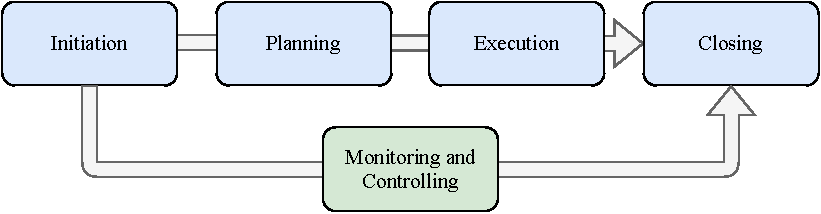
\includegraphics{data/figures/project_lifecycle.pdf}
  \caption{Project Phases}
  \label{fig:projectphases}
\end{figure}


\section{Project Initiation}
\label{ch:projectinitiation}
The project initiation is the first stage of every project. Firstly, the overall goal of the project needs to be defined on a high level. Secondly, the project manager needs to be named. In a project as small as this one, the project manager and the project team are one and the same. Thirdly, the key stakeholders are identified.


\subsection{Project Charter}
\label{ch:projectcharter}
\begin{tcolorbox}
  The overall goal of the project is a well documented implementation of the Advanced Encryption Standard. The end result should be a working piece of software that can encrypt and decrypt some input in the way defined in chapter~\ref{ch:aes}.
\end{tcolorbox}


\subsection{Project Team}
\label{ch:projectteam}
In order for the project to start the group working on the project needs to be defined. As this project (the implementation of the Advanced Encryption Standard) will be carried out by a team of two, all team decisions have to be made at this stage. At the kick-off meeting for the project teams could be formed. After short private conversation the team for this project was decided. A meeting was setup so the first stages of planning could take place. The team for this project are Jan Phillip Berg and Simon Keil.

\subsection{Stakeholders}
\label{ch:stakeholders}
It is crucial for the project's success to identify the stakeholders and their respective interests, involvement and interdependencies. As this is a project carried out in an academic context, the stakeholders are the lecturers grading and reviewing the final work. They not only have a big impact on project success by grading the end result, but will have an involvement throughout the process with regular feedback. This feedback will be gathered through progress presentations given by the project team every two weeks. As there are no other stakeholders, the project team themselves excluded, there are no interdependencies to manage.


\section{Planning Phase}
\label{ch:planningphase}
The planning phase of the project is where the project management plan is created. This section of the thesis contains the definitions of requirements and scope, as well as the management of schedule, communications, and quality.

\subsection{Scope Management}
\label{ch:scopemanagement}
In most projects the "Magic Triangle" of scope, cost and schedule needs to be managed \cite{vanwyngaard2012}. The academic nature of this project removes considerations for cost, simplifying the planning and giving more room for playing with schedule and scope. The scope of a project should be defined as \textit{all} and \textit{only} the work required to complete the project successfully. We will define the scope of this project in the following sections by first listing the requirements. Afterwards, we will give a scope statement.

\subsubsection{Requirements}
\label{ch:requirements}
The high level goal of the project defined in chapter~\ref{ch:projectcharter} can be extended into some more detailed requirements listed below. The requirements are sorted into the those concerning the software's functionality, the implementation, and the documentation of the software.
\paragraph{Requirements on the software:}
\begin{itemize}
  \item encryption of a text input via AES-128 with a given key
  \item decryption of an encrypted text via AES-128 with a given key
  \item computation of all lookup tables used in AES-128
  \begin{itemize}
    \item computation of the SBox
    \item computation of the Round Constants for the key expansion
  \end{itemize}
\end{itemize}

\paragraph{Requirements on the implementation:}
\begin{itemize}
  \item implementation of AES key expansion
  \item separate implementations of en- and decryption
  \item visible and even work-split between team members
  \item steady progress with biweekly presentable results
\end{itemize}

\paragraph{Requirements on the documentation:}
\begin{itemize}
  \item thesis of 20 pages containing:
  \begin{itemize}
    \item theoretical background on symmetric encryption and its use-cases
    \item detailed explanation of the AES algorithm
    \item project plan
  \end{itemize}
  \item program documentation 30 pages containing:
  \begin{itemize}
    \item functions
    \item usage
    \item implementation
    \item performance
  \end{itemize}
\end{itemize}

\subsubsection{Scope Statement}
\label{ch:scopestatement}
\begin{tcolorbox}
  The project of implementing the Advanced Encryption Standard has to goal of creating a software that can encrypt and decrypt text inputs in AES-128 with a given key. Specifically excluded from the scope are the handling of binary input, AES-256 and up, and the unification of en- and decryption functionality into one callable executable. The software has run on one common operating system only. Further compatibility is excluded from the scope. Documentation of the software and explanations of the Advanced Encryption Standard's functionality are to be included.
\end{tcolorbox}


\subsection{Schedule Management}
\label{ch:schedulemanagement}

In order to develop a schedule the activities must be defined. We will use a work breakdown structure for this purpose, which can be found in section~\ref{ch:wbs}. Afterwards, we will sequence the different work packages and assign them to team members.

\subsubsection{Work Breakdown Structure}
\label{ch:wbs}



\section{Execution Phase}
\label{ch:executionphase}

\section{Monitoring and Controlling}
\label{ch:monitoringcontrolling}

\section{Project Closing and Delivery}
\label{ch:projectclosing}


% \bibliography{references.bib} needed to fix autocompletion for citation in my editor
